\documentclass[tikz]{standalone}
\usetikzlibrary{arrows,decorations.markings}

\def\A{(5,0)}
\def\B{(5,4)}
\def\C{(0,4)}

\def\D{(10,0)}
\def\E{(10,4)}
\def\F{(15,4)}

\def\G{(0,9)}
\def\H{(15,9)}

\def\I{(0,6.5)}
\def\J{(15,6.5)}

\def\K{(7.5,0)}
\def\L{(7.5,4)}

\def\M{(5,6.5)}
\def\N{(7.5,6.5)}

\def\UNOb{(0,5.67)}
\def\UNOe{(10.83,5.67)}

\def\DUEb{(0,4.83)}
\def\DUEe{(5.83,3)}

\def\TREb{(15,7.43)}
\def\TREe{(6.67,3)}

\def\QUATTROb{(15,8.17)}
\def\QUATTROe{(3.2,8.17)}

\def\CINQUEb{(8.33,0)}
\def\CINQUEe{(3.2,7.43)}

\def\SEIb{(9.17,0)}
\def\SEIe{(10.83,4.83)}

\begin{document}
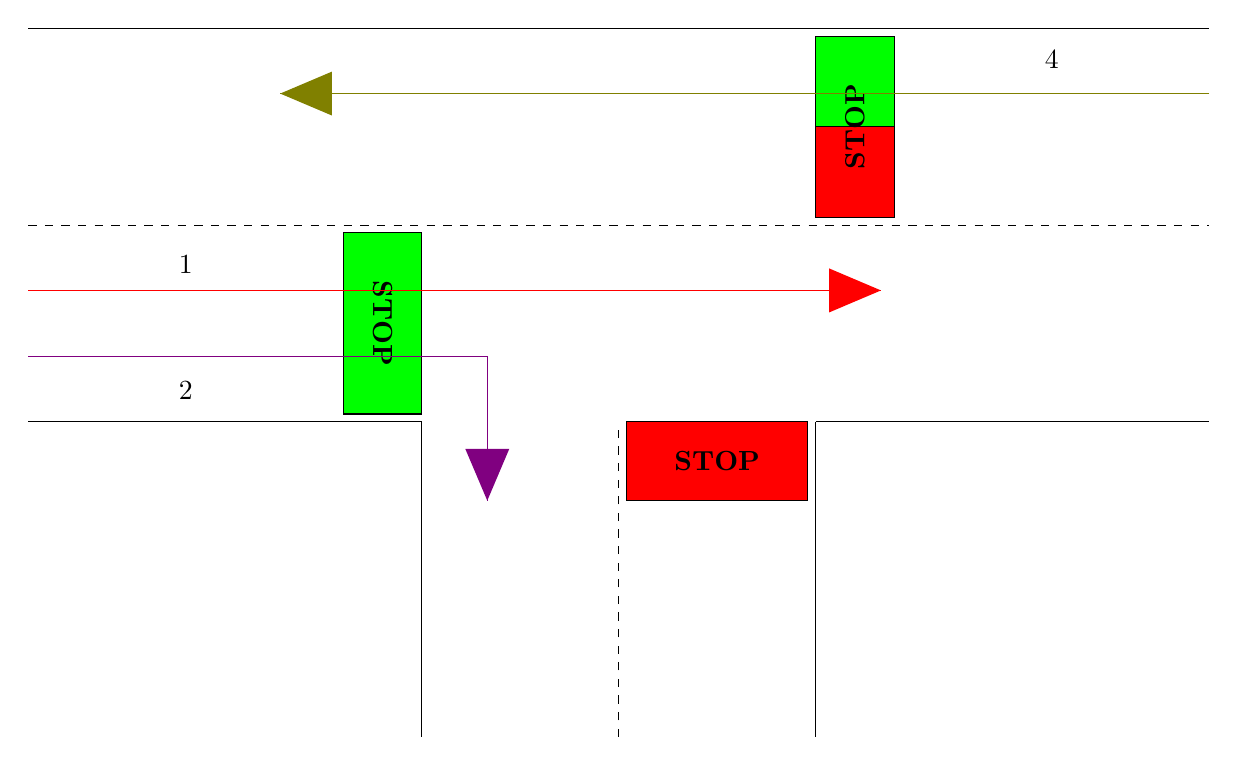
\begin{tikzpicture}[>=triangle 45,
decoration={markings,mark=at position 1 with {\arrow[scale=3]{>}}}]
\draw[fill=green] (5,4.1) rectangle (4,6.4);
\node[rotate=-90] at (4.5,5.25) {\bf {STOP}};
\draw[fill=green] (10,7.75) rectangle (11,8.9);
\draw[fill=red] (10,6.6) rectangle (11,7.75);
\draw (10,6.6) rectangle (11,8.9);
\node[rotate=90] at (10.5,7.75) {\bf {STOP}};
\draw (7.6,4)[fill=red] rectangle (9.9,3);
\node at (8.75,3.5) {\bf {STOP}};

\draw \A -- \B;
\draw \C -- \B;

\draw \D -- \E;
\draw \E -- \F;

\draw \G -- \H;

\draw[dashed] \I -- \J;
\draw[dashed] \K -- \L;

% 1
\draw[postaction={decorate},red] \UNOb -- \UNOe;
\node (uno) at (2,6) {1};

% 2
\draw[postaction={decorate},red!50!blue] \DUEb -| \DUEe;
%  \DUEb .. controls (5.83,4.83) and (5.83,4.) .. \DUEe;
\node (due) at (2,4.4) {2};

% 4
\draw[postaction={decorate},red!50!green] \QUATTROb -- \QUATTROe;
\node (quattro) at (13,8.6) {4};
\end{tikzpicture}
\end{document} 
